\documentclass{article}
\usepackage{polski}
\usepackage[utf8]{inputenc}
\usepackage[toc,page]{appendix}
\usepackage{listings}
\usepackage{enumitem}
\usepackage{graphicx}
\graphicspath{ {obrazy/} }
\author{Wojciech Decker}
\title{Sprawozdanie - implementacja algorytmu LZW}
\begin{document}
\maketitle
\tableofcontents
  \begin{section}{Cel projektu}
    Celem projektu była implementacja i demonstracja zasady działania kompresji LZW
  \end{section}
  \begin{section}{Algorytm}
    LZW - Lempel–Ziv–Welch został zaprezentowany w 1984r. przez panów Abraham'a Lempel, Jacob'a Ziv i Terry'ego Welch.
    Jest słownikowym algorytmem kompresji danych, względnie prostym w implementacji. 
    Pozwala na uzyskanie zadowalających wyników przy niskim koszcie obliczeń. 
    Na co dzień jest z powodzeniem wykorzystywany w systemach UNIX, oraz formacie GIF.

    \begin{subsection}{Kodowanie}
      Podczas kodowania wczytywane porcje danych, w mojej implementacji o długości 8 bitów są tłumaczone na wartości kodów słownika
      Inicjalizacja polega na stworzeniu słownika, zawierającego wszystkie podstawowe słowa i przypisane im kody od 1 w górę.
      Następnie wczytywane kolejno słowa są tłumaczone na kody i sklejane. 
      Jeżeli sklejone kody nie znajdują się w słowniku, są do niego dodawane.

      Dokładny przebieg algorytmu wygląda następująco:
      \begin{enumerate}
	\item Zainicjalizuj słownik słowami o długości 1, przypisując im wartości kodowe.
	\item Znajdź najdłuższe słowo $W$ znajdujące się na wejściu, które znajduje się w słowniku.
	\item Wypisz na wyjście kod przypisany do słowa $W$
	\item Usuń słowo $W$ z wejścia
	\item Dodaj słowo $W$ z dodaną kolejną wartością znajdującą się na wejściu
	  przypisując jej kolejną wartość kodu
	\item Idź do pkt. 2 
      \end{enumerate}
      W rezultacie otrzymujemy ciąg wartości kodowych, które zostają wypisane na wyjściu.
      Duży wpływ na skuteczność kompresji ma sposób zapisu kodów.
      Kody powinny być zapisywane na tylu bitach, ile wymaga najwyższa wartość kodu w słowniku.
      Pozwala to sukcesywnie zwiększać liczbę bitów wymaganych do zapisu kodu, zmniejszając rozmiar pliku wynikowego.
    \end{subsection}
    \begin{subsection}{Dekodowanie}
      Proces dekodowania - dekompresji pliku do postaci oryginalnej przebiega analogicznie do kodowania.
      Tworzony jest identyczny słownik, z tą różnicą, że to wartościom kodów przypisywane są jednoelementowe
	wartości słów.
      Wczytywane są kolejne kody, tłumaczone na ciągi słów, nieznane wcześniej słowa są dodawane do słownika z kolejnymi wartościami kodów.

      Dokładny przebieg algorytmu dekodującego:
      \begin{enumerate}
	\item Zainicjalizuj słownik słowami o długości 1, przypisując im wartości kodowe.
	\item Wczytaj nowy kod $pk$ i przetłumacz na słowo $W$
	\item Wypisz na wyjście słowo $W$
	\item Wczytaj kod $k$ z wejścia 
	\item Przypisz do $pc$ słowo skojarzone z kodem $pk$
	\item Jeśli kod $k$ jest zdefiniowany w słowniku, dodaj do słownika ciąg $pc$ z dopisanym pierwszym znakiem słowa $k$. 
	  Wypisz na wyjście słowo przypisane do $k$.
	\item W przeciwnym wypadku dodaj do słownika ciąg $pc$ z dopisanym pierwszym znakiem słowa $pc$ i wypisz je na wyjście
	\item Do $pk$ przypisz wartość $k$
	\item Idź do pkt. 4
      \end{enumerate}
      Efektem działania algorytmu dekodującego będzie plik identyczny z oryginalnym.
    \end{subsection}
  \end{section}
  \begin{section}{Implementacja}
      Implementacja algorytmu LZW została wykonana w języku Sala działającym na platformie Java.

      Najważniejsze klasy:
      \begin{description}[leftmargin=8em,style=nextline]
	\item[LZW] implementacja wykonania algorytmów na wejściu i wyjściu
	\item[MutableCompression] algorytm kompresji
	\item[MutableDecompression] algorytm dekompresji
	\item[DummyIntWriter] zapisuje kodu o długości 32 bitów w 2, 3 lub 4 segmentach po 8 bitów
	\item[DummyIntReader] odczytuje kody o zapisane w segmentach przez $DIW$ i rzutuje na kod 32 bitowy
      \end{description}

  \end{section}
  \begin{section}{Prezentacja rezultatów}
    \begin{table}[h]
    \begin{tabular}{| l | l | l | l |}
      \hline
      Nazwa pliku		& rozmiar oryginalny	& rozmiar po kompresji& współczynnik kompresji	\\\hline
      \hline
      algorithm.txt		&	4043	&	3320	&	.82117	\\\hline
      lena16.png		&	206871	&	322398	&	1.55844	\\\hline
      lena24.png		&	131864	&	198330	&	1.50404	\\\hline
      lena48.png		&	61866	&	91776	&	1.48346	\\\hline
      lena64.png		&	42263	&	65394	&	1.54731	\\\hline
      lena8.png			&	389740	&	608799	&	1.56206	\\\hline
      lena.png			&	511937	&	796173	&	1.55521	\\\hline
      pan-tadeusz.txt		&	493390	&	263472	&	.53400	\\\hline
      pismo\_swiete.txt		&	5389056	&	2340807	&	.43436	\\\hline
      short.txt			&	7	&	12	&	1.71428	\\\hline
    \end{tabular}
    \caption{Tabela wyników kompresji}
    \end{table}
    %\begin{figure}[h]
    %  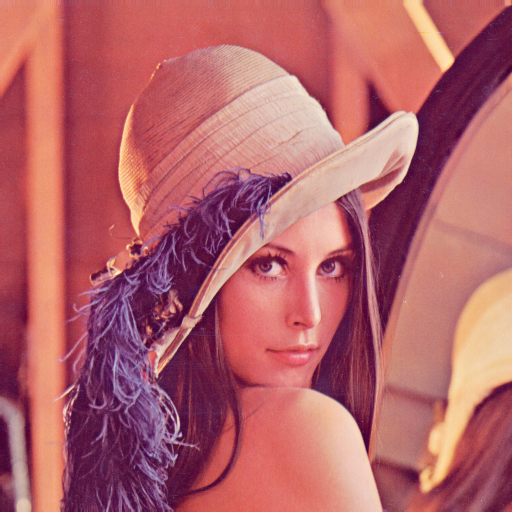
\includegraphics[width=\textwidth]{lena}
    %  \caption{Lena}
    %\end{figure}
    Kompresję przeprowadzono na plikach tekstowych i graficznych. 
    Implementacja generuje kody 32 bitowe, zapisując je w segmentach 8-bitowych, pomijając zapis
    zbędnych segmentów zerowych. 
    Algorytm okazał się najwydajniejszy dla dużych plików tekstowych.
    Dla krótkiego tekstu \textit{algorithm.txt} zawierającego fragment opisu algorytmu z anglojęzycznej wikipedii
    współczynnik kompresji wyniósł 82\%.
    Tekst dłuższy - \textit{Pan Tadeusz} - Adama Mickiewicza po kompresji miał 53\% rozmiaru oryginalnego.
    Kompresja Biblii, będącej najdłuższym tekstem dała współczynnik kompresji 43\%.

    Implementacja została przetestowana pod kątem kompresji obrazów graficznych różnych rozmiarów.
    Kompresja grafiki dawała współczynnik kompresji na stałem poziomie ok. 154 \%.
  \end{section}
  \begin{section}{Wnioski}
    Kompresja daje największy zysk dla długich plików tekstowych. 
    Kompresja obrazów przynosi skutek odwrotny do zamierzonego.
    Przyczyną małej wydajności kompresji może być sposób alokacji bitów do zapisu kodu, 
    operujący na blokach 8-bitowych zamiast na pojedynczych bitach.
  \end{section}
  \begin{section}{Załączniki}
  \appendix
    \begin{section}{Algorytm kompresji}
      \lstinputlisting[breaklines=true,caption={Algorytm kompresji}]{MutableCompression.scala}
    \end{section}
    \begin{section}{Algorytm dekompresji}
      \lstinputlisting[breaklines=true,caption={Algorytm kompresji}]{MutableDecompression.scala}
    \end{section}
  \end{section}
\end{document}
